\chapter{Аналитический раздел}
\label{cha:analysis}
%\chapter{Аналитический раздел}\label{sec:analyth}

%В данном разделе формализована поставленная задача и описаны общие требования и допущения, рассмотрены основные модели данных, поддерживаемые СУБД, а также рассмотрены существующие реализации поставленной задачи. 

\section{Формализация поставленной задачи}

Задачей данной курсовой является разработка базы данных для хранения и анализа данных некой медицинской компании, а также соответствующего приложения, предоставляющего интерфейс для работы с базой.

Предметной областью поставленной задачи является деятельность некоторой медицинской клиники. Для автоматизации учета информации разрабатывается т.н. медицинская информационная система. Под этим термином можно понимать любую информационную систему, которая хранит и обрабатывает информацию, связанную со здоровьем пациентов и деятельностью учреждений здравоохранения\cite{def}.

Основными трудностями при разработке МИС являются:

\begin{itemize}
	\item трудности, связанные с государственным документооборотом, конфиденциальностью персональных данных и врачебной тайной\cite{troubles};
	\item в рамках развития интегрированных медицинских информационных систем возрастает роль готовности медицинского персонала и пациентов к участию в этих процессах\cite{ready}. Большинство врачей практически не владеют компьютерными технологиями, поэтому им проще вести бумажные ведомости, чем использовать программное обеспечение, что приводит к существенному снижению эффективности работы клиники.
\end{itemize}

\clearpage
\subsection*{Общие требования к разрабатываемому программному обеспечению}

Предметная область поставленной задачи является обширной и включает в себя множество понятий и связей между ними, в связи с этим были сформулированы следующие требования к разрабатываемой программе в рамках курсовой работы:

\begin{itemize}
	\item должен быть предоставлен функционал для регистрации и аутентификации пользователей в системе, также должен быть создан личный кабинет с основной информацией о пользователе;
	\item должен быть предоставлен функционал для записи пациента на прием к врачу, а также отслеживания как активных, так и обработанных заявок. Должна формироваться медицинская карта с возможностью ее просмотра;
	\item должна быть предоставлена статистика по заболеваемости среди зарегистрированных случаев в данной клинике.
\end{itemize}

Также были сформулированы следующие допущения:

\begin{itemize}
	\item в рамках курсовой работы не затрагивается тема контроля врачебной тайны и  конфиденциальности персональных данных пациента. Таким образом, любой доктор может просмотреть все данные из медицинской карты пациента;
	\item в разрабатываемой МИС отсутствует платежная система, т.е. нельзя проводить и фиксировать финансовые транзакции;
	\item МИС не ведет складской учет (инвентаризация, маркировка медикаментов и т.д.);
	\item не предусматривается возможность отмены заявки на прием. В конечном итоге заявка должна быть одобрена специалистом;
	\item разрабатываемая МИС предоставляет функционал только для администрирования приемов клиентов докторами клиники, для администрирования сведений в медицинской карте пациента, а также предоставляет возможность сбора и отображения статистики обращений в клинику.
\end{itemize}

\clearpage

\subsection*{Формализация данных}

На рисунке 1.1 представлена диаграмма сущность-связь в нотации Чена\cite{erm}, описывающая сущности предметной области и их взаимодействие.

\begin{figure}[!h]
	\center{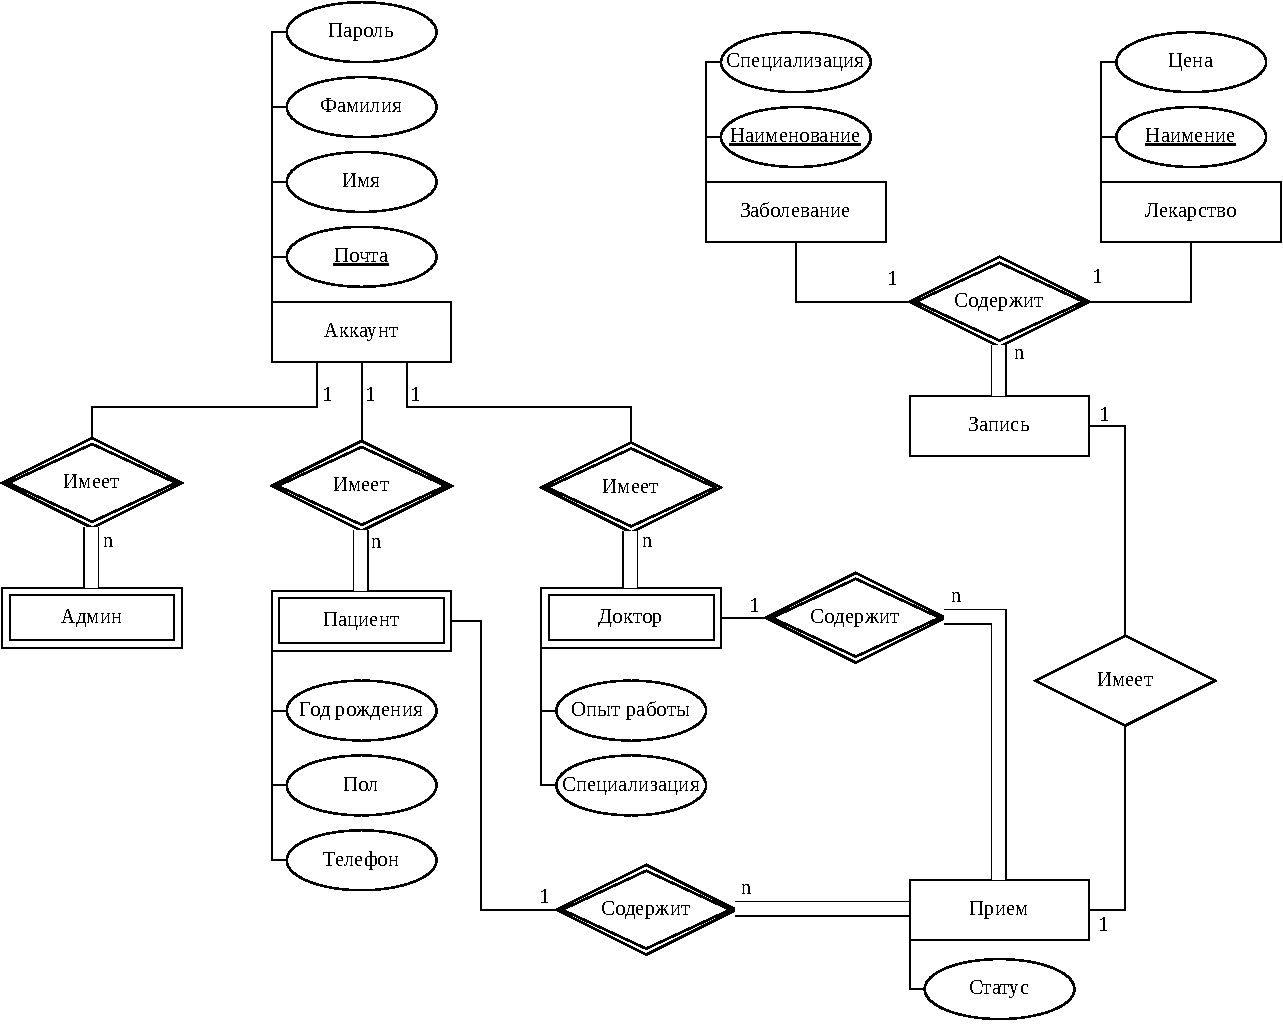
\includegraphics[scale=0.77]{assets/erm2.pdf}}
	\caption{Диаграмма сущность-связь в нотации Чена, описывающая сущности предметной области и их взаимодействие}
\end{figure}

Медицинская информационная система, проектируемая в ходе выполнения курсовой работы, включает в себя информацию о следующих объектах:

\begin{enumerate}
	\item Запись медицинской карты - сущность, описывающая конкретный прием, поставленный диагноз и лекарство для лечения пациента. Набор таких сущностей образуют медицинскую карту пациента.
	\item Прием - сущность, характеризующая поход пациента к врачу. Прием имеет статус, который может принимать одно из двух возможных значений: <<Активный>> (запланированный, еще не совершившийся) и <<Обработанный>> (совершившийся прием).
	\item Диагноз - сущность, описывающая диагноз, который может быть поставлен пациенту. Каждому диагнозу поставлена в соответствие определенная специальность доктора, характеризующая сферу болезни.
	\item Лекарство - сущность, описывающая медикаментозные средства, которые могут быть назначены пациенту.
	\item Аккаунт - сущность общего вида, описывающая каждый из трех возможных подтипов сущностей-пользователей в системе: пациент, доктор или администратор.
\end{enumerate}

\section{Системы управления базами данных}

Система управления базами данных --- совокупность программных и лингвистических средств общего или специального назначения, обеспечивающих управление созданием и использованием баз данных\cite{sbd}.

%Основные функции СУБД\cite{ssbd}:
%
%\begin{itemize}
%	\item Непосредственное управление данными во внешней памяти;
%	\item Управление буферами оперативной памяти;
%	\item Управление транзакциями;
%	\item Журнализация изменений;
%	\item Резервное копирование и восстановление базы данных после сбоя;
%	\item Поддержка языков БД.
%\end{itemize}

Классифицировать СУБД можно, используя различные признаки классификации, например, по степени распределенности, по способу доступа к БД и т.д. Важнейшим классификационным признаком СУБД является тип модели данных, поддерживаемый СУБД.

\subsection*{Классификация СУБД на основе типа модели данных}

\subsubsection*{Дореляционная модель данных}

\textit{Иерархические модели} имеют древовидную структуру, где каждому узлу соответствует один сегмент, представляющий собой поименованный линейный кортеж полей данных. Каждому сегменту соответствует один входной и несколько выходных сегментов. 

Каждый элемент структуры лежит на единственном иерархическом пути, начинающемся от корневого. Модель допускает только два типа связей между сущностями: <<один к одному>> и <<один ко многим>>.

\textit{Сетевая модель} данных является расширением иерархической и призвана устранить ограничения, связанные с ней. В иерархических структурах запись-потомок должна иметь в точности одного предка; в сетевой структуре данных потомок может иметь любое число предков.

Сетевая и иерархическая модели данных тесно связаны с физическим размещением информации.

	%\subsubsection*{Графовая модель данных}

%Графовая модель является подвидом сетевой модели данных и используется для представления текста. Граф определяется как конечное множество объектов (вершин) и множество пар различных вершин (ребер). Такие модели используются преимущественно в гуманитарных областях знаний для автоматической обработки текстов, информационного поиска, стилистической диагностики и т.п\cite{graph}.

\subsubsection*{Реляционная модель данных}

Реляционная модель данных представляет собой совокупность данных, состоящую из набора двумерных таблиц. В теории множеств таблице соответствует термин отношение (relation), физическим представлением которого и является таблица. 

Таблица состоит из строк, называемых записями, и столбцов, называемых полями. На персечении строк и столбцов находятся конкретные значения данных. В таблице не должно быть одинаковых строк, каждый столбец должен иметь уникальное значение.

Эта модель является логической, в отличие от иерархической и сетевой. Она опирается на такие разделы математики, как теория множеств и логика первого порядка.

\subsubsection{Постреляционная модель данных}

Данная модель является расширением реляционной модели. Она снимает ограничение неделимости данных, допуская многозначные поля, и набор значений воспринимается как самостоятельная таблица, встроенная в главную таблицу\cite{postrel}.

\textit{Многомерная модель} представляет данные как многомерные массивы (гиперкубы), использование которых позволяет получать различные срезы при аналитической обработке данных. Осями многомерной системы координат служат основные атрибуты анализируемого бизнес-процесса. На пересечениях осей измерений находятся данные, количественно характеризующие процесс, — меры\cite{postrel2}.

\textit{Объектно-ориентированная модель} представляет из себя структуру, которую графически можно изобразить в виде дерева, узлами которого являются объекты. Базовыми понятиями являются: объекты, классы, методы, наследование, полиморфизм, инкапсуляция.

\subsection*{Выбор модели данных}

Для решения поставленной задачи была выбрана реляционная модель данных, т.к. разрабатываемая база данных характеризуется большим набором отношений между сущностями, и в связи с этим схема базы данных, основанной на этой модели, будет более наглядна и проста, чем аналогичная схема сетевых и иерархический моделей, т.к. в данном случае описание базы данных основывается только на естественной структуре данных без введения какого-либо дополнительного уровня абстракции для их представления. Это свойство обусловлено использованием теории множеств.

%Для решения поставленной задачи была выбрана реляционная модель данных, т.к. база данных характеризуется большим набором отношений (в терминах теории множеств) между сущностями, а задача предполагает постоянное добавление и чтение данных из хранилища. Также реляционная модель не содержит ограничений, свойственных СУБД, основанных на иерархическом и сетевом типе модели данных.

\section{Методы защиты информации}

Выделяют несколько основных уровней защиты информации в базах данных:

\begin{enumerate}
	\item Защита на уровне хранилища. Одним из методов защиты на этом уровне является шифрование -  преобразование некого осмысленного текста в неосмысленный набор символов посредством применения некоторой шифрующей функции\cite{def-online}.
	\item Защита на уровне базы данных. Одним из методов защиты на этом уровне является установление паролей. Пароли устанавливаются пользователями или администраторами системы. Учет и управление паролями выполняется самой СУБД\cite{def-book}\cite{ops}.
	\item Защита на уровне приложения. Процесс предоставления доступа к БД осуществляется путем выполнения регистрации или аутентификации, а затем авторизации в системе. Вход в систему открывает доступ к БД и соответствующим правам авторизированного пользователя.
\end{enumerate}

%В данной курсовой работе необходимо уделить особое внимание обеспечению безопасности системы в виду специфики предметной области.

%\subsection*{Защита паролем}
%
%Наиболее простой и наименее эффективный способ защиты данных. Пароли устанавливаются пользователями или администраторами системы. Каждому пользователю обычно предоставляются различные права доступа. Обычно разные пользователи обладают различными правами доступа к одному и тому же объекту. Учет и управление паролями выполняется самой СУБД\cite{def-book}.
%
%\subsection*{Разграничение прав доступа}
%
%Каждому объекту назначается некий классификационный уровень прав доступа к другим объектам базы данных. Права доступа определяют возможные операции над объектами: удаление, чтение, запись, добавление новых записей\cite{ops}.
%
%Этот метод защиты также не гарантирует полную защиту данных, т.к. злоумышленники может попытаться проникнуть в БД не с помощью средств системы (механизма авторизации), а минуя систему, т.е. перемещая внешние носители информации или подключаясь к линии связи.
%
%\subsection*{Шифрование}

%%Наиболее эффективный способ защиты информации. 
%Под шифрованием понимается преобразование некого осмысленного текста в неосмысленный набор символов посредством применения некоторой шифрующей функции\cite{def-online}. 

%В данной курсовой работе с помощью средств СУБД необходимо обеспечить шифрование на уровне хранилища.

\section{Обзор существующих реализаций}

\subsection*{Medesk}

Данная МИС позволяет проводить мониторинг работы медицинского центра. Система поддерживает складской учет, имеет внутреннюю платежную систему, представляет механизм для тайм-менеджемента, колл-центра и др.
Как и многих систем подобного рода, у Medesk отсутствует бесплатная версия программного обеспечения. Средняя стоимость подписки составляет 3500 рублей в месяц по состоянию на 2022 год.

Данная система представлена на следующих платформах: Web-приложение, Windows, MacOS, Linux.

На рисунке 1.2 представлен пользовательский интерфейс МИС Medesk.

\begin{figure}[!h]
	\center{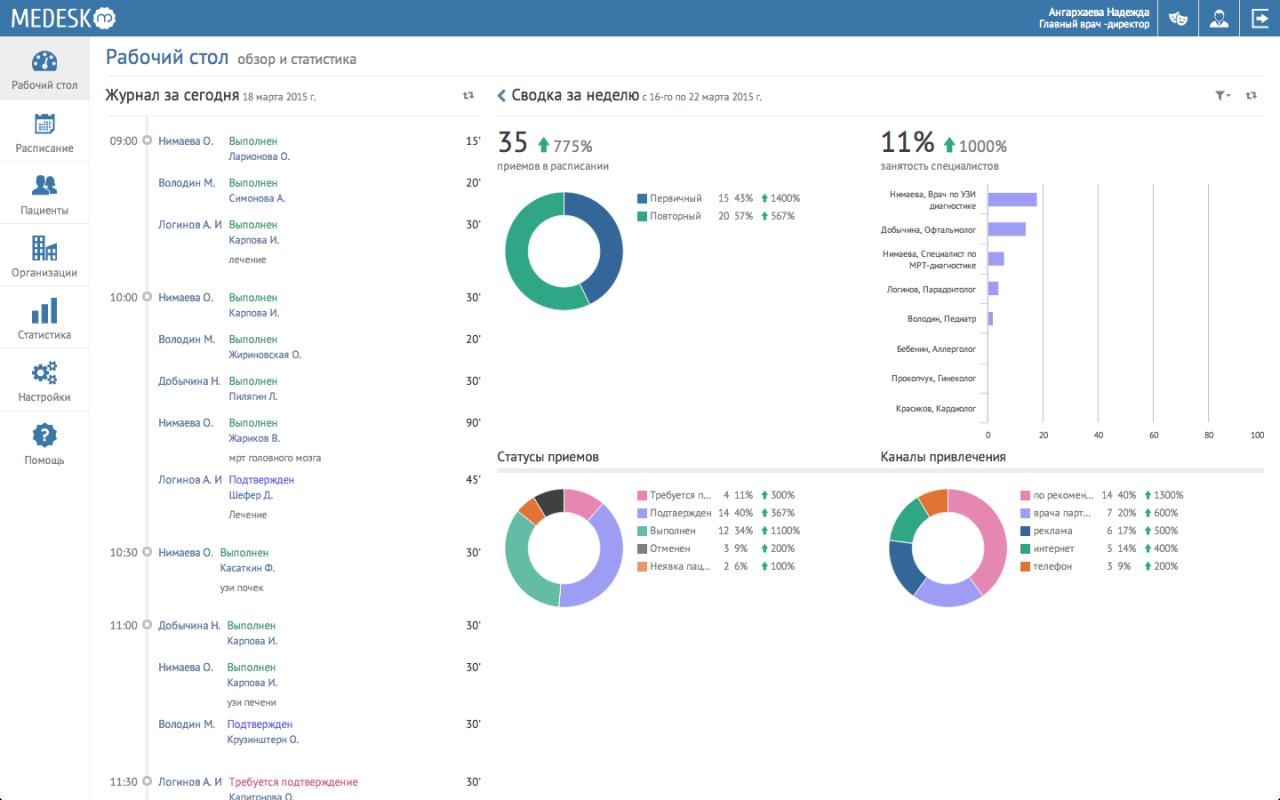
\includegraphics[scale=0.42]{assets/medesk}}
	\caption{Интерфейс МИС Medesk}
\end{figure}

\subsection*{Medods}
 
Программное обеспечение специализировано на стомоталогических клиниках, но в общем случае может предоставлять базовый функционал для любых типов медицинских клиник. 

На рисунке 1.3 представлен пользовательский интерфейс МИС Medods.

\begin{figure}[!h]
	\center{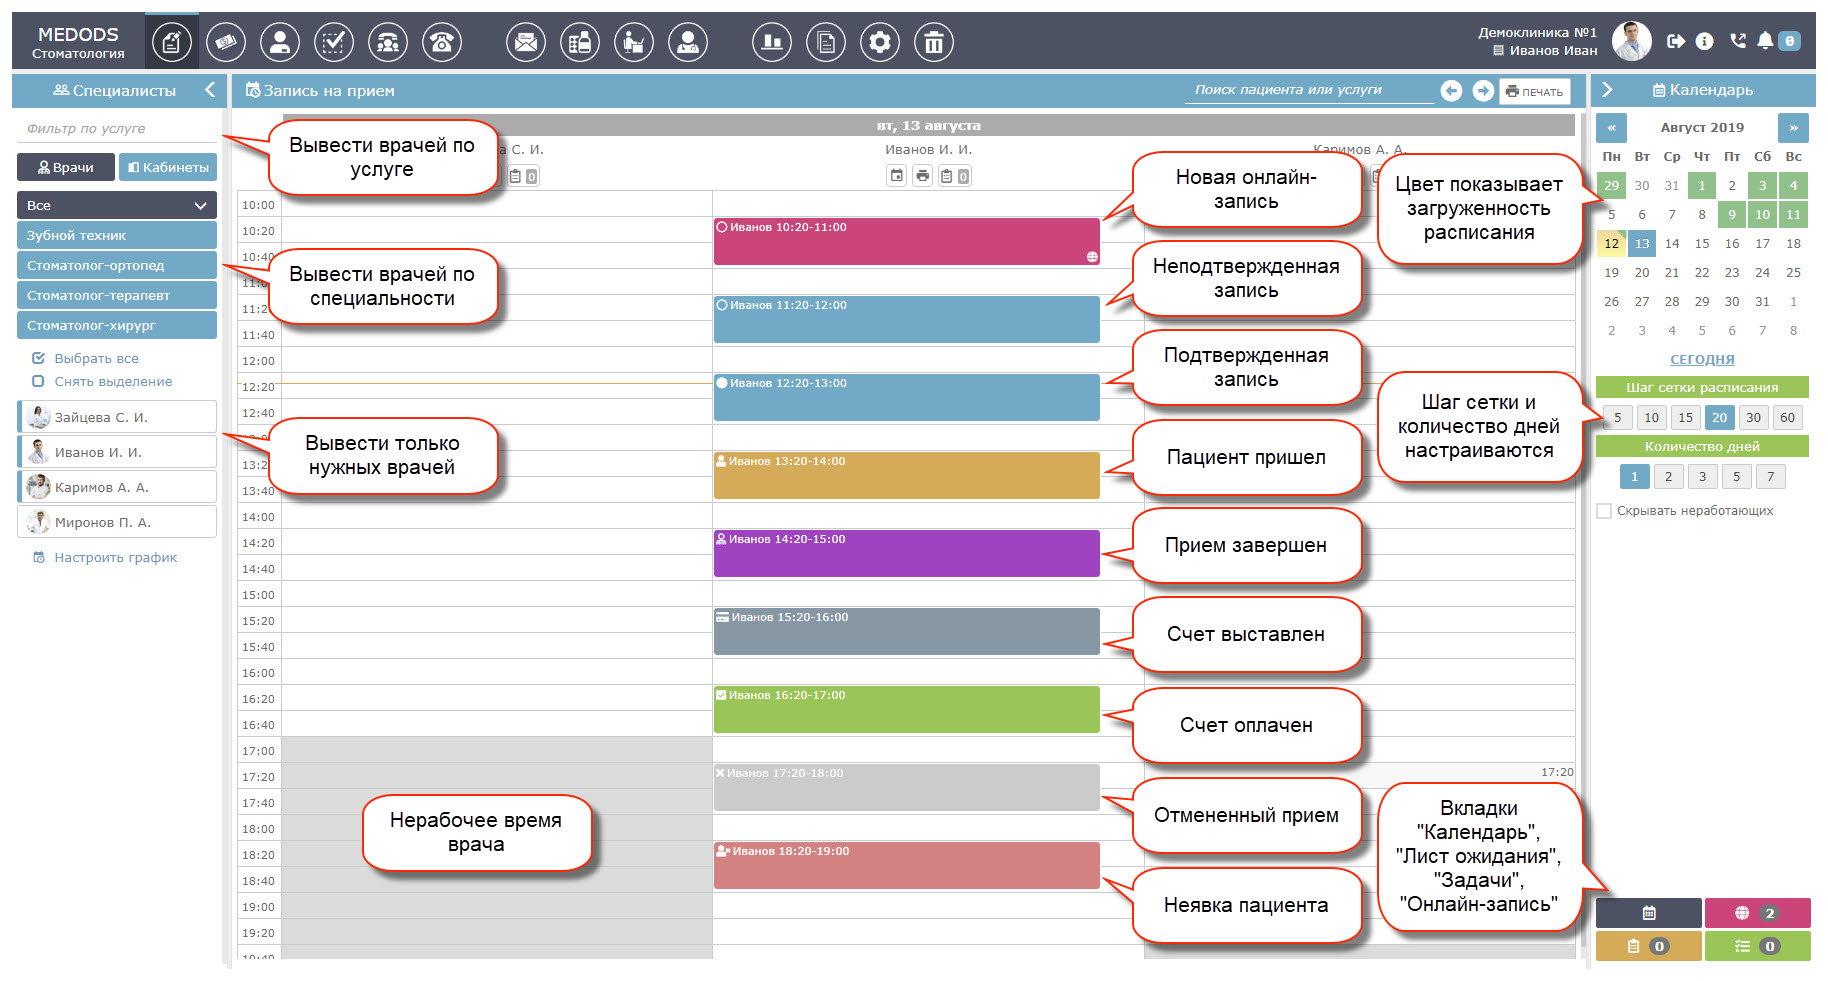
\includegraphics[scale=0.65]{assets/medods}}
	\caption{Интерфейс МИС Medods}
\end{figure}

ПО предоставляет функционал для управления регистратурой, имеет кабинет врача и руководителя, также предоставляет механизм для онлайн-записи на прием и технической поддержки. Система также имеет платежную систему. 

У данного продукта также отсутствует бесплатная версия. Средняя стоимость подписки составляет 4900 рублей в месяц по состоянию на 2022 год.

Данная система представлена на следующих платформах: Web-приложение, Windows, MacOS, Linux. 

\subsection*{Инфоклиника}

Данная МИС предоставляет функционал для многопрофильных клиник. В зависимости от потребностей и особенностей клиники, компания конфигурирует ПО для каждой компании индвидуально и поставляет его заказчикам. Соответственно, у этой МИС также нет бесплатной версии, а средняя стоимость подписки зависит от типа поставляемого ПО.

На рисунке 1.4 представлен пользовательский интерфейс МИС Инфоклиника.

\begin{figure}[!h]
	\center{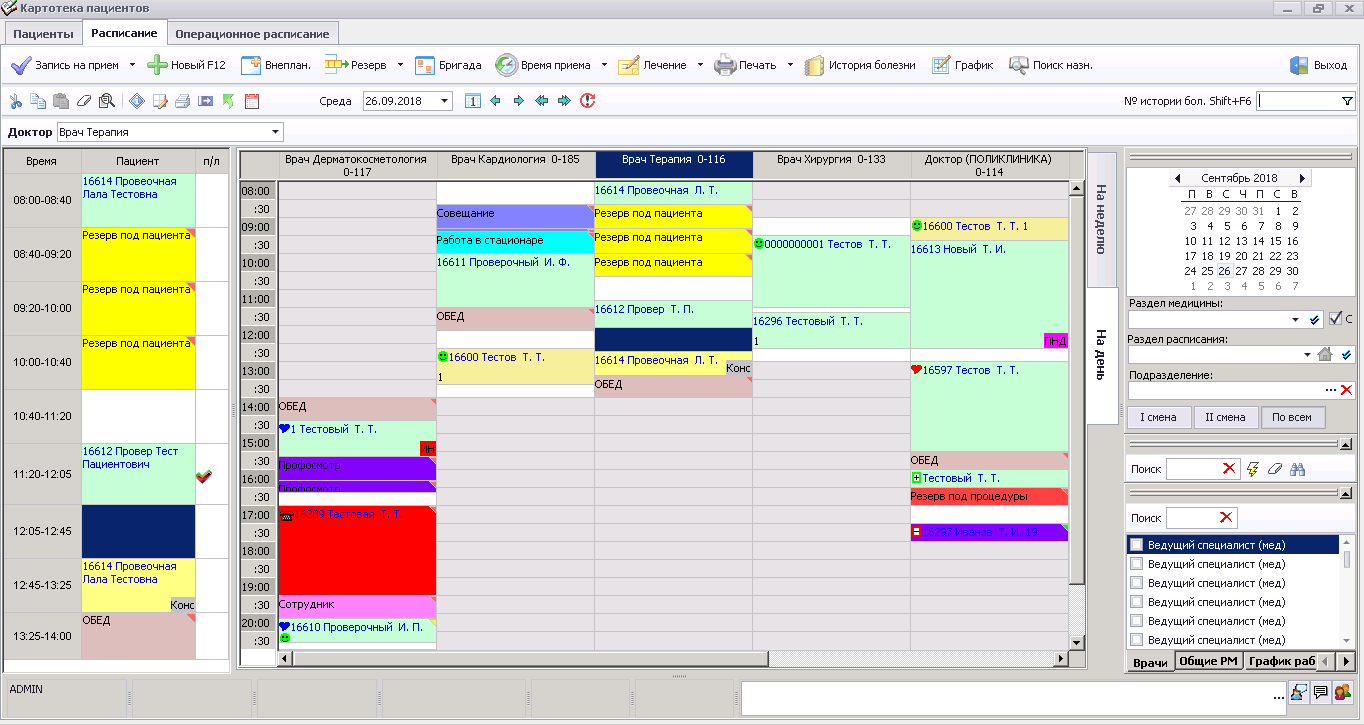
\includegraphics[scale=0.33]{assets/infoclinic}}
	\caption{Интерфейс МИС Инфоклиника}
\end{figure}

Инфоклиника предоставляет широкий функционал: особое внимание уделено созданию мессенджера внутри системы, предоставляется механизм для ведения складского учета, проведения платежей, система предоставляет функционал для страхования.

Данная система представлена на следующих платформах: Web-приложение, Windows. 

\subsection*{Сравнительный анализ существующих реализаций}

В таблице 1.1 представлен сравнительный анализ существующих реализаций. Анализ был проведен в соответствии со следующими критериями:

\begin{itemize}
    \item стоимость - критерий, определяющий является ли ПО бесплатным;
    \item профиль - является ли приложение многопрофильным с точки зрения предоставляемых услуг;
    \item кабинет - возможность создать аккаунт в системе пациентом самостоятельно;
    \item заявка - возможность оставить заявку на прием самостоятельно;
    \item карта - возможность ведения медицинской амбулаторной карты пациента.
\end{itemize}

\begin{table}[h!]
	\begin{center}
	    \caption{Сравнительный анализ существующих реализаций}
		""\newline
		\begin{tabular}{|c|c|c|c|c|c|}
			\hline
			Реализация & Стоимость & Профиль & Кабинет & Заявка & Карта\\[0.8ex]
			\hline
			Medesk & - & + & + & + & + \\
			\hline
			Medods & - & - & + & - & + \\
			\hline
			Инфоклиника & - & + & - & - & - \\
			\hline
		\end{tabular}
	\end{center}
\end{table}	

Обычно ПО подобного рода ориентировано больше на администраторский функционал, чем на пользовательский. Разрабатываемое ПО будет ориентировано на функционал пациента в большей степени, чем это сделано в рассмотренных реализациях: пациент будет иметь возможность самостоятельно создать аккаунт в системе, самостоятельно оставить заявку на прием, посмотреть заявки и медицинскую историю (карту), будет сформирован личный кабинет. Также разрабатываемое ПО будет распространяться бесплатно и будет многопрофильным.

\section*{Вывод}

В данном разделе была формализована поставленная задача, сформулированы общие требования и допущения к разрабатываемому ПО, проведен обзор существующих реализаций. Были рассмотрены модели хранения данных и для решения поставленной задачи была выбрана реляционная модель.	